\documentclass{chinese-journal-of-mechanical-engineering}

\addbibresource{../refs/bib/references.bib}
\ExecuteBibliographyOptions{doi=false,url=false,eprint=false}

\doi{}
\setcounter{secnumdepth}{2}
\renewcommand{\thesection}{\arabic{section}}
\renewcommand{\thesubsection}{\arabic{section}.\arabic{subsection}}
\AtBeginBibliography{\clubpenalty=10000\widowpenalty=10000\interlinepenalty=10000}

\renewcommand{\InfoBundle}{%
    \title{智能结构等几何优化综述}%
    \author[1]{xx}%
    \affil[1]{xx}%
    \abst{等几何分析采用统一样条基函数同时描述 CAD 几何与分析场，为结构尺寸、形状和拓扑优化提供了几何建模、数值分析与灵敏度计算一体化框架。面向复杂壳体、曲边胞元和增材制造轻量化构件，传统“几何重建-网格再生-优化更新”流程往往存在模型转换频繁、边界质量受限和设计变量语义不一致等问题；等几何分析能够在统一几何表示下组织分析求解、优化更新和几何回写，为高保真结构优化提供技术基础。本文聚焦智能结构优化设计场景，综述等几何分析在结构优化中的主要进展。首先介绍 B 样条、NURBS 与等几何离散的基本表达，并概述 SIMP 材料插值、伴随灵敏度、滤波正则化、水平集演化和自由形变映射等经典模型；随后从密度法、水平集法、移动可变形构件和多补丁壳结构优化等路线梳理等几何拓扑优化与形状优化的代表性工作；最后讨论超材料、点阵结构、增材制造、智能生成和开源工作流等融合趋势。现有研究表明，复杂多补丁几何、局部细化、可制造性约束、几何回写以及数据驱动方法与物理模型的耦合，仍是推动该方向工程应用的关键问题。
}%
    \keyword{等几何分析；结构优化；形状优化；拓扑优化；壳结构}}

\renewcommand{\EnInfoBundle}{%
    \title{A Review of Isogeometric Optimization for Intelligent Structures}%
    \author[1]{xx}%
    \affil[1]{xx}%
    \abst{Isogeometric analysis employs unified spline basis functions to describe CAD geometry and analysis fields, thereby providing an integrated framework for geometric modeling, numerical analysis and sensitivity evaluation in size, shape and topology optimization. For complex shells, curved cellular structures and additive-manufactured lightweight components, conventional workflows based on repeated geometry reconstruction, remeshing and optimization updates often suffer from frequent model transfer, limited boundary quality and inconsistent design-variable semantics. Isogeometric analysis can organize analysis, optimization updates and geometry feedback within a unified geometric representation, which provides a technical basis for high-fidelity structural optimization. This review focuses on isogeometric analysis for intelligent structural optimization. It first introduces the basic B-spline/NURBS formulation and isogeometric discretization, and then summarizes classical models including SIMP material interpolation, adjoint sensitivity analysis, filtering regularization, level-set evolution and free-form-deformation parameterization. Representative routes for isogeometric topology and shape optimization are reviewed from density-based methods, level-set methods, moving morphable components and multi-patch shell optimization. Recent trends in metamaterials, lattice structures, additive manufacturing, intelligent generation and open-source workflows are further discussed. Existing studies indicate that complex multi-patch geometries, local refinement, manufacturability constraints, geometry feedback and the coupling between data-driven methods and physics-based models remain key issues for engineering applications.
}%
    \keyword{isogeometric analysis; structural optimization; shape optimization; topology optimization; shell structures}}

\begin{document}

\hypersetup{
    colorlinks=true,
    linkcolor=black,
    citecolor=black,
    urlcolor=black
}

\maketitle
\thispagestyle{firststyle}

\begin{multicols}{2}
\linespread{1.24}\selectfont
\setcounter{section}{-1}
\section{前言}

结构优化设计旨在在满足强度、刚度、稳定性和制造约束的前提下，合理分配材料、调整结构边界或优化关键尺寸，从而提升结构综合性能。按照设计变量不同，相关研究通常可划分为尺寸优化、形状优化和拓扑优化三类\cite{Wu2021SMO}。传统有限元方法虽然较为成熟，但在复杂曲面边界、薄壁壳体拓扑以及频繁几何更新场景下，几何重建、网格生成和分析模型维护仍然构成主要瓶颈。

等几何分析将 CAD 中常用的 B 样条、NURBS、细分曲面和 T 样条基函数直接用于数值分析，使几何表示与计算模型保持一致，从而减少“设计模型”与“分析模型”之间的转换损失\cite{Wang2021FMEReconstruction,Wen2024CompStructPHT,Liu2018CJSolid}。这种 CAD/CAE 一体化特征使其适合结构优化问题：设计变量可以直接定义在控制点、厚度场或密度场上，高阶连续基函数也有利于曲面边界更新、壳体弯曲分析和灵敏度计算。

近年来，等几何结构优化已从参数化曲线曲面问题扩展到多补丁壳体、自由形变驱动厚度优化以及非结构 T 样条支撑下的形状-拓扑协同优化\cite{Bandara2019ArXiv,Zhao2024EngComput,Wang2025CADA}。本文围绕等几何分析在智能结构优化设计中的方法进展与工程应用展开，重点讨论其在几何建模、拓扑优化、壳结构优化和智能生成闭环中的作用，并归纳现有问题与未来方向。

\section{等几何分析与结构优化基础}

\subsection{CAD/CAE 一体化思想}

等几何分析的核心思想，是采用与 CAD 几何一致的样条基函数同时完成几何描述与数值离散，从而减少传统有限元流程中几何重建、网格生成和模型映射带来的信息损失\cite{Wang2021FMEReconstruction,Pan2024CADMultiPatch}。对于结构优化而言，这种一体化框架的意义不只是提高几何精度，更在于把设计变量、物理响应和优化更新放入同一参数空间中。控制点可以作为形状变量，厚度场可以依附于曲面参数域，密度场也可以用样条函数连续表示，由此形成从 CAD 建模到 CAE 分析再到优化回写的闭环。近期壳结构形状-拓扑同步优化研究也指出，B 样条或 NURBS 不仅能够精确表达几何边界，还便于建立形状灵敏度和优化模型，这为后续等几何结构优化提供了方法基础\cite{Zhang2024CompStruct}。

以一维 B 样条为例，其 Cox--de Boor 递推关系可写为
\begin{equation}
\begin{aligned}
N_{i,0}(\xi)&=
\begin{cases}
1, & \xi_i \le \xi < \xi_{i+1},\\
0, & \text{otherwise},
\end{cases}\\
N_{i,p}(\xi)&=\frac{\xi-\xi_i}{\xi_{i+p}-\xi_i}N_{i,p-1}(\xi)
+\frac{\xi_{i+p+1}-\xi}{\xi_{i+p+1}-\xi_{i+1}}N_{i+1,p-1}(\xi) .
\end{aligned}
\label{eq:bspline}
\end{equation}
NURBS 进一步引入控制点权重，其有理基函数为
\begin{equation}
R_{i,p}(\xi)=\frac{N_{i,p}(\xi)w_i}{\sum_{j=1}^{n}N_{j,p}(\xi)w_j} .
\label{eq:nurbs_basis}
\end{equation}
几何映射与位移近似可由同一组基函数统一表示为
\begin{equation}
\mathbf{x}=\sum_A R_A\mathbf{P}_A,\qquad
\mathbf{u}^h=\sum_A R_A\mathbf{d}_A .
\label{eq:iga_map}
\end{equation}
式\eqref{eq:iga_map} 表明，控制点既承载几何形状，也参与分析离散。近期等几何形状优化研究已经证明，在这种统一表示下，几何映射、刚度矩阵和目标函数对设计变量的导数能够稳定传递\cite{Kim2021Symmetry}。

\begin{figure}[H]
    \centering
    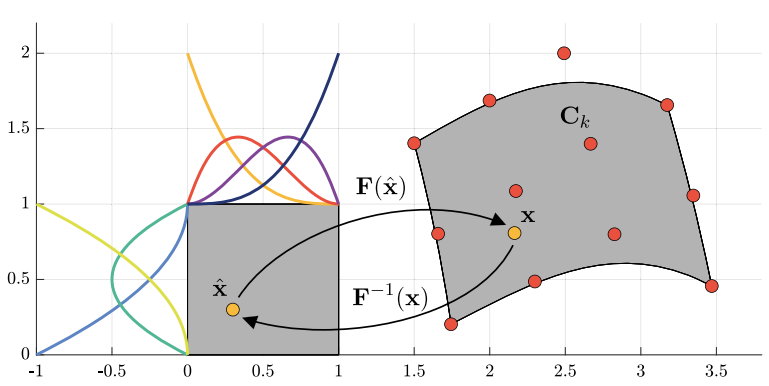
\includegraphics[width=0.96\columnwidth]{../assets/fig_nurbs_mapping.png}
    \caption{二维 NURBS 曲面从参数域到物理域的映射}
    \label{fig:nurbs_mapping}
\end{figure}

图\ref{fig:nurbs_mapping} 展示了参数域到物理域的映射关系。与传统有限元中几何模型和分析网格分离的流程相比，等几何分析可以在控制网层面直接更新结构外形，因此特别适合复杂曲面、薄壁壳体和边界敏感结构。近年来，除张量积 NURBS 外，T 样条、PHT 样条和 THB 样条也被用于解决局部细化、多补丁连接和复杂边界表达问题\cite{Zhang2024CMATsplines,Wen2023ArXivPHT,Zhu2023CMESTHB}。

\subsection{结构优化模型}

结构优化通常包括尺寸优化、形状优化和拓扑优化三类。三者的差别在于设计变量不同：尺寸优化主要调整厚度、截面或材料参数；形状优化改变边界或中面几何；拓扑优化则改变材料分布和连接关系\cite{Mei2021Buildings,GaoQiang2024JME}。对于智能结构优化设计，三类问题往往并不是孤立存在，而是在概念设计、方案细化和制造校核阶段依次或交替出现。尤其在运载装备、航空结构和多物理场承载构件中，拓扑优化往往承担早期构型探索任务，而形状和尺寸优化则更多服务于局部细化、强度校核和制造修正。

\begin{figure}[H]
    \centering
    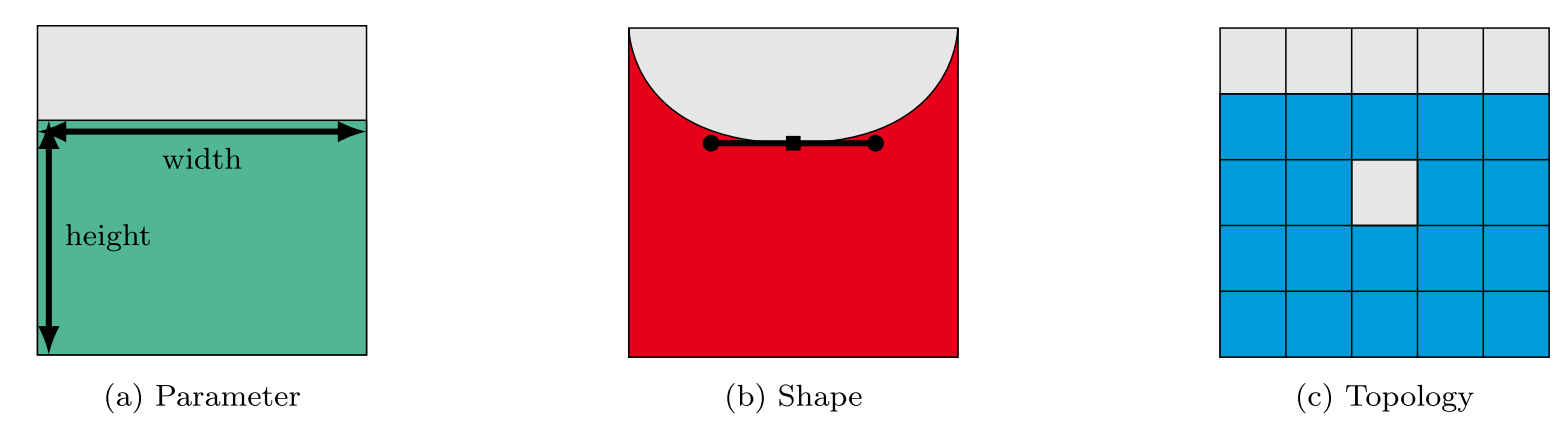
\includegraphics[width=\columnwidth]{../assets/fig_structural_types_added.png}
    \caption{结构优化的基本类型}
    \label{fig:structural_types}
\end{figure}

图\ref{fig:structural_types} 概括了结构优化的基本类型。在拓扑优化中，柔顺度最小化和体积分数约束是最常见的基准模型。SIMP 材料插值可写为
\begin{equation}
\begin{aligned}
E(\rho)&=E_{\min}+\rho^p(E_0-E_{\min}),\\
0&<\rho_{\min}\le \rho \le 1 .
\end{aligned}
\label{eq:simp}
\end{equation}
对应的优化问题为
\begin{equation}
\begin{aligned}
\min_{\rho}\quad & c(\rho)=\mathbf{U}^{\mathrm{T}}\mathbf{K}(\rho)\mathbf{U} \\
\text{s.t.}\quad & \mathbf{K}(\rho)\mathbf{U}=\mathbf{F},\\
& V(\rho)/V_0 \le f .
\end{aligned}
\label{eq:topopt}
\end{equation}
式\eqref{eq:simp}--\eqref{eq:topopt} 是密度法拓扑优化的基础，也被广泛移植到等几何设计空间中\cite{WangChao2021SMO,Qian2013CMA}。当设计变量为几何参数 $a$ 时，柔顺度的一阶灵敏度通常可写为
\begin{equation}
\frac{\partial c}{\partial a}
=-\mathbf{U}^{\mathrm{T}}\frac{\partial \mathbf{K}}{\partial a}\mathbf{U} .
\label{eq:adjoint}
\end{equation}
该式体现了伴随灵敏度分析在形状优化和厚度优化中的基础作用。等几何方法的优势在于，几何变量、分析变量和灵敏度变量具有一致的参数化来源，因此可降低反复网格重构带来的误差和成本\cite{Kiendl2014CMA}。在应力约束和动态响应问题中，这种优势更加明显：基于 IGA-SIMP 的应力约束拓扑优化可以利用高阶连续基函数改善应力计算质量，而面向简谐激励结构的等几何拓扑优化则进一步说明，材料场级数展开与等几何分析结合后，可在动力学目标下保持较少设计变量和较平滑的材料分布\cite{LiuHongliang2018CJCM,WangPeijin2024CJCM}。

\section{等几何拓扑优化研究进展}

\subsection{密度法与多尺度设计}

密度法仍然是等几何拓扑优化中应用最广的路线。与传统单元密度法相比，等几何密度法通常在参数域中以连续样条场描述材料分布，因而可以减轻棋盘格、锯齿边界和后处理困难等问题\cite{Gao2019IJNME,Wen2024CompStructPHT}。Qian 将拓扑优化直接置于 B 样条设计空间中，提出用连续样条变量替代逐单元密度变量\cite{Qian2013CMA}；Kang 和 Youn 进一步将这一思想用于修剪 NURBS 壳结构，说明复杂 CAD 边界也可以参与材料布局优化\cite{Kang2016FEAD}。从国内近期研究看，运载工程结构、三维薄壁填充结构以及复杂热流承载结构的优化设计，均显示出拓扑优化正在由标准二维算例转向大规模、强约束和工程工况驱动的实际问题\cite{GaoQiang2024JME,Bai2024JME,LiBaotong2024JME}。

为了控制最小特征尺寸并提高可制造性，密度法通常需要滤波或投影。Helmholtz 型滤波方程可写为
\begin{equation}
-r^2\nabla^2 \tilde{\rho}+\tilde{\rho}=\rho ,
\label{eq:helmholtz_filter}
\end{equation}
其中 $\rho$ 为原始密度，$\tilde{\rho}$ 为滤波后密度，$r$ 为滤波半径。该思想与等几何分析强调连续表示和边界平滑的目标一致。Wang 等结合多层网格、MGCG 求解器和局部更新策略，提高了高分辨率等几何拓扑优化效率\cite{Wang2019AdvEngSoft}；Gao 等将等几何拓扑优化用于回入型和手性 auxetic 结构，说明曲边连续表示对负泊松比超材料的几何质量和性能实现具有重要作用\cite{Gao2019CMAAuxetic}。对于多尺度问题，循环对称结构和点阵散热结构的中文研究表明，B 样条参数化、等效性能插值和各向异性材料插值可以共同降低微结构设计变量数量，并提高单胞连续过渡和热学性能定制能力\cite{Zhang2021CJCM,Xiao2024JME}。

\begin{figure}[H]
    \centering
    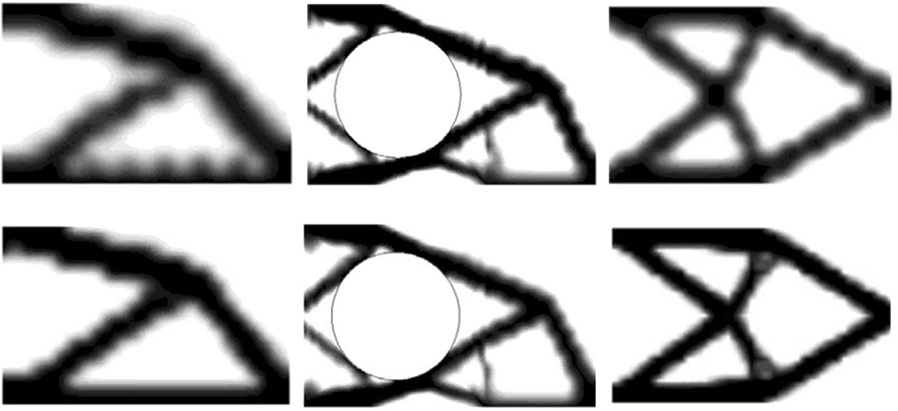
\includegraphics[width=\columnwidth]{../assets/fig_topopt_results.png}
    \caption{密度法等几何拓扑优化结果}
    \label{fig:topopt_results}
\end{figure}

图\ref{fig:topopt_results} 反映出等几何密度法在边界平滑方面的优势。对于增材制造、胞元结构和轻量化构件，优化结果是否具有可重构边界和可制造特征，往往与目标函数数值同样重要。近期针对热弹性多构型梯度点阵、热力耦合拓扑优化和流-热-力耦合结构的研究说明，工程结构的优化目标已从单一刚度或质量指标扩展到热、流、力多场共同约束下的综合性能设计\cite{WangQi2024HKXB,Zheng2024JME,LiRongqi2024CME}。

\subsection{水平集法与显式参数化}

水平集法通过隐式函数跟踪结构边界，适合获得黑白分明的拓扑结果。其边界演化方程通常为
\begin{equation}
\frac{\partial \phi}{\partial t}+V_n|\nabla \phi|=0 ,
\label{eq:levelset}
\end{equation}
其中 $\phi$ 为水平集函数，$V_n$ 为法向演化速度。Xu 等将水平集法用于基频最大化的等几何拓扑优化，H\"ubner Scherer 等进一步将其扩展到曲厚壳和非匹配多补丁结构，说明该路线正在从规则平面连续体走向复杂工程壳体\cite{Xu2019FME,HubnerScherer2024CMA}。Teixeira 等从拓扑导数角度研究等几何边界插入与孔洞萌生，为显式边界演化提供了新的灵敏度机制\cite{Teixeira2025ArXivTD}。

图\ref{fig:levelset_domain} 说明，水平集法适合表达孔洞生成、合并与边界移动。与之相近，移动可变形构件（MMC）方法使用可移动、可伸缩、可旋转的参数化构件描述结构，将拓扑变化转化为显式几何参数优化。Hou 等构建了基于 MMC 的显式等几何拓扑优化框架，Xie 等进一步引入 R-functions 与配置点策略改进构件布尔运算和边界融合\cite{Hou2017CMA,Xie2018CMA}。参数化水平集方法和移动可变形孔洞方法的中文研究也表明，显式或半显式几何描述有利于减少设计变量、提高边界可解释性，并在微结构和超弹性结构设计中表现出较好的适应性\cite{Wei2021CJCM,Xue2019CJCM}。

\begin{figure}[H]
    \centering
    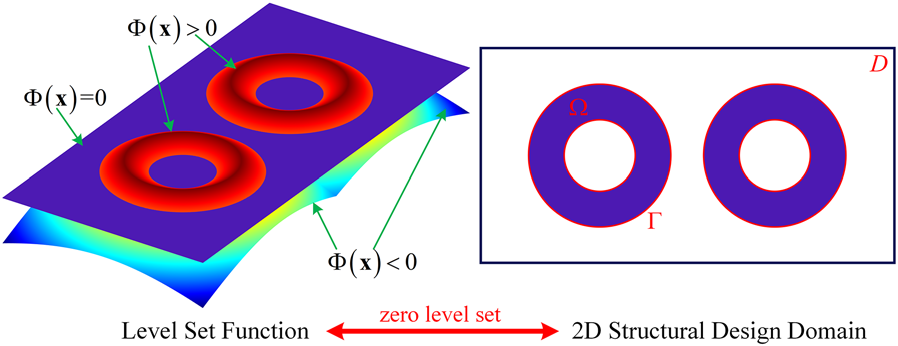
\includegraphics[width=0.94\columnwidth]{../assets/fig_level_set_design_domain.png}
    \caption{水平集边界演化示意}
    \label{fig:levelset_domain}
\end{figure}

图\ref{fig:mmc_results} 展示了显式构件参数化方法得到的典型拓扑形态。与密度云图相比，MMC 结果中的构件边界和连接关系更容易被设计人员理解，也更便于在后处理阶段转化为可编辑几何。

\begin{figure}[H]
    \centering
    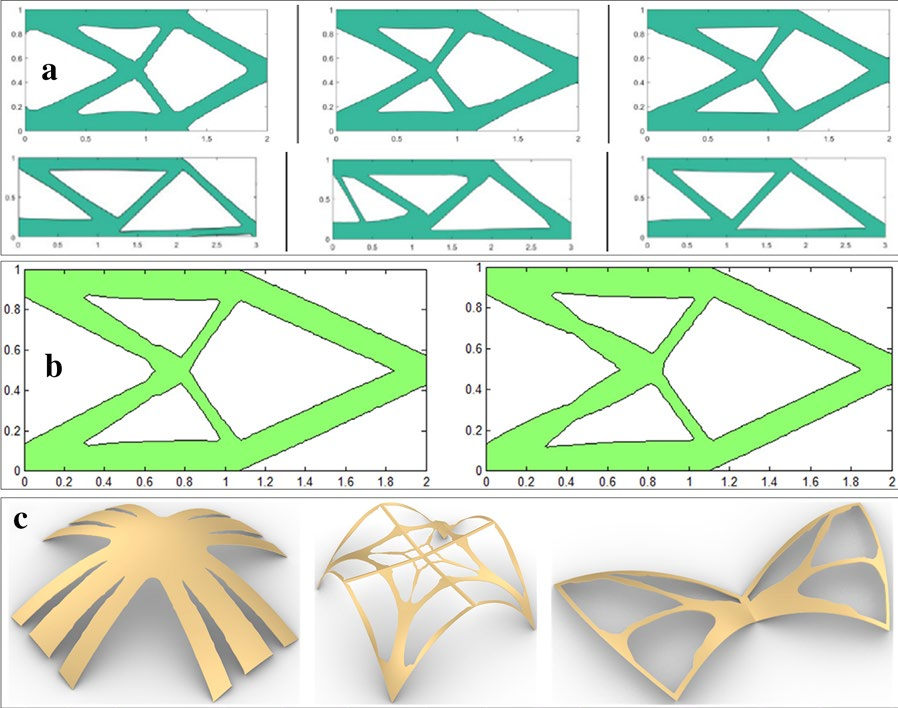
\includegraphics[width=\columnwidth]{../assets/fig_mmc_results.png}
    \caption{MMC 显式拓扑优化结果}
    \label{fig:mmc_results}
\end{figure}

\begin{table}[H]
    \caption{代表性等几何结构优化方法比较}
    \label{tab:method_compare}
    \centering
    \scriptsize
    \setlength{\tabcolsep}{2.8pt}
    \renewcommand{\arraystretch}{1.14}
    \begin{tabular}{p{0.17\columnwidth}p{0.18\columnwidth}p{0.28\columnwidth}p{0.18\columnwidth}}\toprule
        方法路线 & 设计变量 & 主要特点 & 代表研究 \\\midrule
        密度法/SIMP & 连续密度场 & 实现成熟，适合多尺度和高分辨率设计 & \cite{Gao2019IJNME,Wang2019AdvEngSoft} \\
        水平集/拓扑导数 & 隐式边界函数 & 边界清晰，适合孔洞演化和黑白设计 & \cite{Xu2019FME,HubnerScherer2024CMA,Teixeira2025ArXivTD} \\
        MMC/显式参数化 & 构件几何参数 & 变量较少，便于制造约束和工程解释 & \cite{Hou2017CMA,Xie2018CMA,Xue2019CJCM} \\
        局部细化样条 & T/PHT/THB 样条 & 局部加密能力强，适合复杂边界更新 & \cite{Zhang2024CMATsplines,Wen2023ArXivPHT,Zhu2023CMESTHB} \\\bottomrule
    \end{tabular}
\end{table}

表\ref{tab:method_compare} 表明，不同路线的根本差别在于设计变量和边界表达方式。密度法更适合概念布局，水平集法和 MMC 更适合清晰边界，局部细化样条则有利于复杂几何区域的局部精化。实际工程中常需要组合使用这些路线，而不是简单选择单一算法。

从文献评价角度看，等几何拓扑优化的研究不能只按算法名称分类，还应结合设计阶段和工程对象判断其适用性。密度法的优点是模型成熟、收敛经验丰富，适合快速获得材料分布趋势，但优化结果通常仍需要阈值化、边界重构和制造修正；水平集法边界更清晰，但孔洞萌生、重新初始化和复杂曲面上的界面演化会增加实现难度；MMC 方法天然具有构件语义，便于把杆件、孔洞、加强筋等结构特征转化为参数变量，但当构型非常复杂时，构件数量和初始布置会影响最终结果。等几何分析在这些路线中的共同作用，是提供连续、可编辑、可回写的几何底座，使优化结果更容易从“数值密度图”转化为工程设计对象。

此外，中文近年文献反映出一个明显趋势：拓扑优化问题正在从理想边界条件下的标准算例转向热、流、力、振动和制造约束共同作用的工程对象\cite{LiBaotong2024JME}。这意味着方法评价不能只比较目标函数下降幅度，还需要讨论边界条件是否接近实际工况、约束是否覆盖制造过程、优化后模型是否能够直接进入 CAD/CAE 流程。对等几何方法而言，这些问题正好对应其几何参数化优势，也决定了其未来能否从学术算例走向工程软件。

\section{壳结构优化与智能融合趋势}

\subsection{多补丁壳体与形状优化}

薄壁壳体、屋盖、拱壳和机电耦合构件通常具有复杂曲面和多补丁连接，传统有限元形状优化容易受到网格畸变和几何重构影响。等几何分析因具有高阶连续性和 CAD 原生参数化，在壳结构形状优化中表现出明显优势。Kiendl 等针对典型薄壳建立了半解析灵敏度和灵敏度加权策略，Bandara 和 Cirak 基于细分曲面提出多分辨率壳体形状优化方法，均说明平滑曲面表达能够提高形状更新稳定性\cite{Kiendl2014CMA,Bandara2019ArXiv}。相关综述进一步指出，等几何结构优化的前沿问题包括剪裁 CAD 几何、实体几何构造、壳体优化、材料和结构一体化优化以及不确定性优化，这些问题恰好对应工程设计中最难保持几何一致性的环节。

近年来，多补丁和非匹配几何成为研究重点。Zhao 等利用自由形变（FFD）盒体统一管理多个 NURBS 壳补丁的形状和厚度变量，并通过罚函数与 Lagrange extraction 处理补丁不匹配问题\cite{Zhao2024EngComput}。其 FFD 映射可写为
\begin{equation}
\mathbf{x}(\xi,\eta,\zeta)=\sum_{i=0}^{l}\sum_{j=0}^{m}\sum_{k=0}^{n}
B_i^l(\xi)B_j^m(\eta)B_k^n(\zeta)\mathbf{P}_{ijk}.
\label{eq:ffd_map}
\end{equation}
式\eqref{eq:ffd_map} 表明，复杂壳体可由较少的外部控制点完成整体变形，从而降低设计变量维数。随后，相关工作又将移动交线问题纳入优化过程，并给出基于 FEniCS 与 OpenMDAO 的开源流程，为复杂壳体优化的可复现研究提供了基础\cite{Zhao2024ArXivIntersections,Zhao2024ArXivOpenSource}。

\begin{figure}[H]
    \centering
    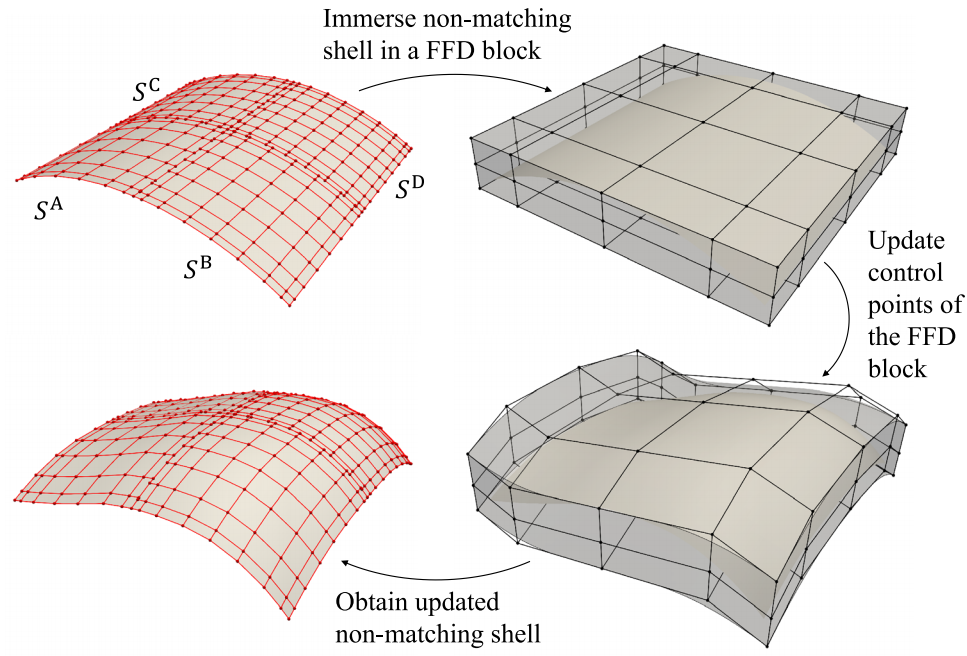
\includegraphics[width=\columnwidth]{../assets/workflow_ffd_shape_optimization.png}
    \caption{FFD 壳结构优化流程}
    \label{fig:ffd_workflow}
\end{figure}

图\ref{fig:ffd_workflow} 展示了壳结构优化的典型闭环：由 CAD 曲面和 FFD 控制框架定义设计变量，通过等几何壳体分析获得响应和灵敏度，再将更新后的参数回写到几何模型。Wang 等基于分析适配非结构 T 样条实现了 Kirchhoff--Love 壳结构的形状-拓扑一体化优化，说明复杂壳面拓扑更新、光滑边界重建和高质量分析离散可以在同一框架内协同完成\cite{Wang2025CADA}。结合国内热力耦合结构优化研究可以看出，等几何分析的潜在应用对象已经从纯力学壳结构扩展到多材料、多工况和多物理场系统\cite{Zheng2024JME}。

壳结构优化还涉及一个常被忽视的问题，即优化变量的物理意义。若直接移动大量有限元节点，虽然能够改变外形，但节点位移未必对应清晰的设计参数，优化后的模型也难以被设计人员继续修改。等几何方法把控制点、节点矢量、权重、厚度场和局部变形框架作为变量，使形状变化具有更明确的几何语义。对于屋盖、机匣、翼肋和复杂曲面支撑结构，这种语义保留有助于把“算法得到的最优形状”转化为“工程人员可解释和可调整的设计方案”。因此，等几何壳结构优化的价值不仅在于计算精度，也在于保留设计知识和后续编辑能力。

\subsection{数据驱动设计与工程闭环}

智能结构优化并不意味着用黑箱模型替代物理模型，而是利用代理模型、参数化几何、制造知识和高保真校核提升候选方案搜索效率。对于等几何结构优化而言，数据驱动方法最适合承担初始构型生成、代理评价和参数预筛选任务，而最终方案仍需回到力学控制方程、制造约束和 CAD 可编辑性中接受检验。多尺度点阵和流-热-力耦合结构的中文研究表明，工程应用最关心的并不是单个算法名称，而是候选构型能否在力学、热学、制造和几何回写之间保持一致\cite{Xiao2024JME}。

\begin{figure}[H]
    \centering
    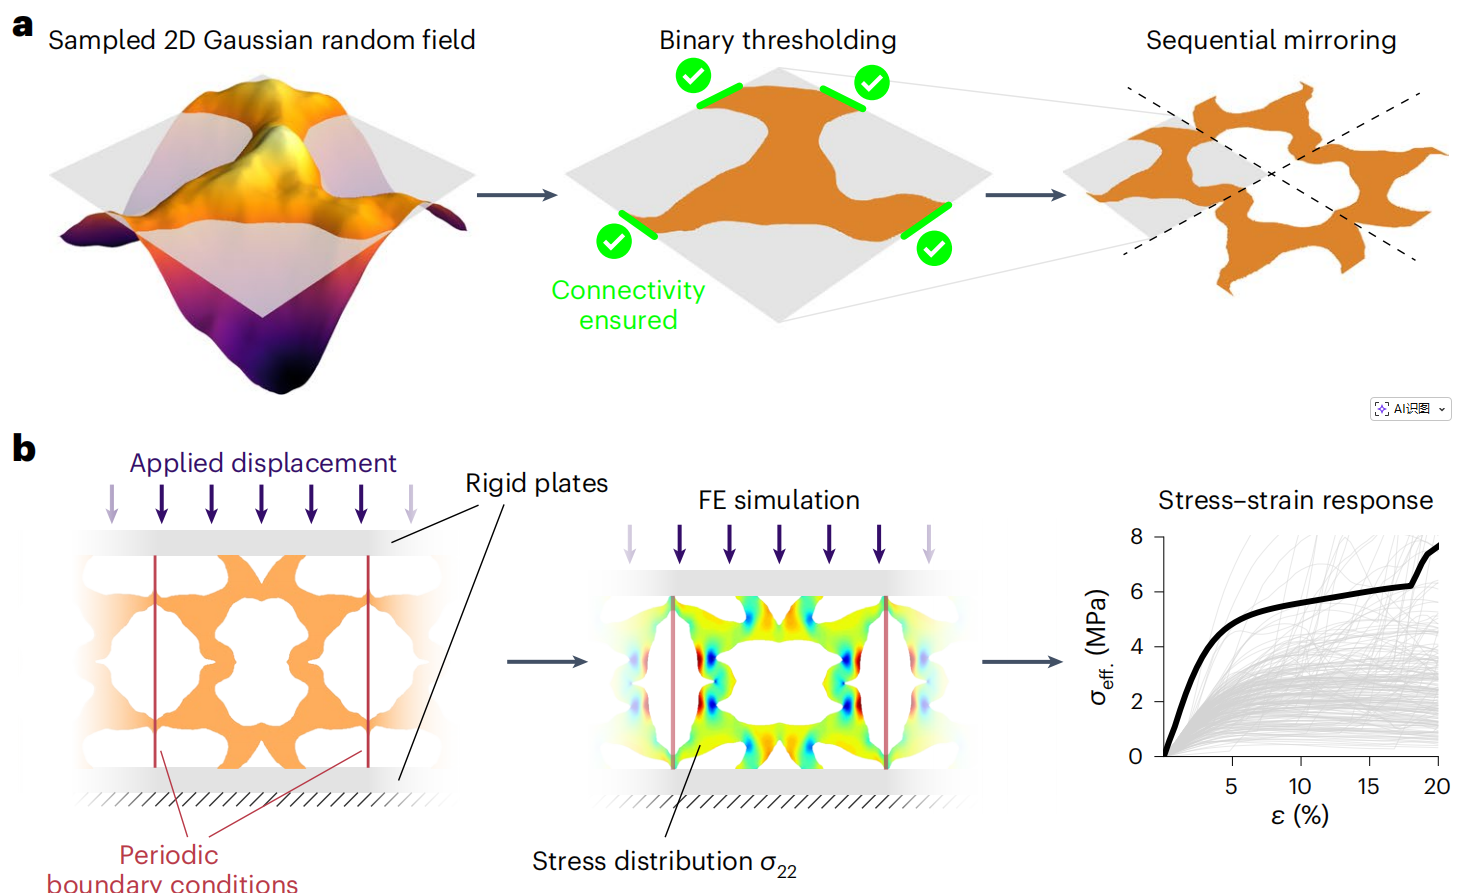
\includegraphics[width=\columnwidth]{../assets/metamaterial_generation_process.png}
    \caption{机械超材料智能生成与性能校核流程}
    \label{fig:meta_generation}
\end{figure}

图\ref{fig:meta_generation} 概括了智能生成方法在结构优化中的基本位置：数据模型先给出候选胞元或拓扑形态，随后仍需要通过物理仿真、制造约束和几何回写进行筛选。对于曲边超材料和点阵结构，这种流程与等几何分析的连续几何表达具有较好的互补性。

在等几何框架内引入智能方法，一个合理路径是“先生成、再校核、后回写”：生成模型或代理模型先给出候选拓扑，等几何分析再执行高保真物理校核和灵敏度修正，最后将结果转化为可编辑几何。Hu 等基于 pix2pix 的多补丁等几何拓扑优化工作即体现了这种思路，即利用图像到图像模型快速预测候选结构，再保留等几何分析作为物理校核环节\cite{Hu2023FrontPhys}。与只输出像素化拓扑图相比，这一路径更强调设计变量语义、曲面连续性和制造约束的同步保留。

\begin{table}[H]
    \caption{智能结构优化闭环中等几何分析的作用}
    \label{tab:intelligent_loop}
    \centering
    \scriptsize
    \setlength{\tabcolsep}{2.8pt}
    \renewcommand{\arraystretch}{1.14}
    \begin{tabular}{p{0.14\columnwidth}p{0.21\columnwidth}p{0.20\columnwidth}p{0.22\columnwidth}}\toprule
        环节 & 输入信息 & 输出结果 & 等几何分析作用 \\\midrule
        几何建模 & CAD 曲面、控制点、厚度参数 & 样条几何模型 & 保持精确几何和设计变量语义 \\
        物理求解 & 载荷、边界、材料属性 & 位移、应力、频率响应 & 提供高连续离散和稳定灵敏度 \\
        智能生成 & 数据集、代理模型、生成模型 & 候选拓扑或形状 & 提供可校核、可回写的几何表达 \\
        工程闭环 & 制造约束、后处理接口 & 可编辑 CAD/CAE 模型 & 支撑参数回写和方案复用 \\\bottomrule
    \end{tabular}
\end{table}

表\ref{tab:intelligent_loop} 说明，等几何分析在智能设计中的主要价值在于连接 CAD、CAE、优化器和数据模型，并为智能结构优化提供统一参数化框架。要形成可靠平台，仍需在开放基准、数据格式、制造约束和可复现工作流方面继续完善\cite{Wu2021SMO,Zhao2024ArXivOpenSource,Wen2022LXXB}。

为了使不同研究具有可比性，后续文献还需要采用更统一的评价维度，包括力学性能、几何质量、制造一致性和工作流完整性。若只比较目标函数值，容易忽略后处理成本；若只展示拓扑图形，又难以判断结构是否真正可制造。等几何分析的研究优势，应通过这些综合指标体现出来。

从数据资产角度看，智能结构优化所需的数据不应只是最终结构图片，还应包含控制点、节点矢量、材料参数、边界条件、载荷工况、目标函数、约束函数、迭代历史和制造标签等信息。等几何模型天然保存几何参数与分析变量之间的对应关系，因此适合作为高质量结构优化数据集的组织形式。围绕典型壳体、点阵材料和热力耦合构件建立开放数据集，将有助于推动物理优化方法与智能生成方法的公平比较。

\subsection{当前问题与发展方向}

综合已有研究，等几何结构优化面临三类突出问题。第一，复杂 CAD 模型中的多补丁连接、移动交线和局部细化规则仍不统一，导致几何一致性和数值稳定性难以同时保证\cite{Zhao2024ArXivIntersections}。第二，多尺度胞元、增材制造和多物理场耦合问题带来更高维度的设计变量和更复杂的约束，现有求解器效率、灵敏度传递和后处理流程仍需改进\cite{Bai2024JME,WangQi2024HKXB}。第三，数据驱动方法的泛化能力和物理一致性依赖高质量数据资产，而当前公开数据集往往缺少控制网、边界条件、优化历史和制造标签等完整信息。

因此，未来研究应从单一算法竞争转向系统工作流建设，建立面向多补丁壳体、曲边超材料和机电耦合构件的统一几何表示、局部细化和参数回写机制，并把力学性能、几何可编辑性、制造一致性、计算效率和模型泛化能力纳入统一评价体系。只有当优化结果能够在性能、几何和制造三个层面同时闭合，等几何分析才真正能够支撑智能结构优化设计的工程落地。

综上，等几何分析在结构优化中的作用可概括为“几何一致性驱动的优化平台”。未来研究应更加重视稳健参数化与局部细化、多物理场与制造约束前置，以及开源代码、开放数据和标准算例支撑下的可复现研究。

\section{总结与展望}

本文围绕智能结构优化设计场景下的等几何分析研究，对统一几何-分析描述、结构优化经典数学模型以及密度法、水平集法、MMC 和多补丁壳体优化等主要技术路线进行了综述。综合全文，主要认识如下。

（1）等几何分析的核心价值并不局限于高阶离散本身，而在于以统一样条模型贯通 CAD 建模、结构分析和优化更新，使拓扑优化、形状优化与厚度优化能够共享同一几何基础。

（2）从方法与应用进展看，等几何结构优化已由规则连续体问题扩展到多补丁壳体、壳型胞元、超材料以及与增材制造协同的复杂轻量化结构；同时，数据驱动设计、智能生成和几何回写也在重塑结构优化的实现路径。

（3）当前研究仍存在复杂几何参数化、局部细化、多尺度建模、可制造性约束以及数据驱动与物理模型耦合不足等问题。后续研究应进一步建立开放基准、统一数据格式和可复现工作流，使不同算法能够在相同几何、载荷、约束和制造条件下进行比较。

从工程应用角度看，等几何分析的价值最终要落实到设计流程中，即优化结果不仅应具有较优性能，还应服务于概念设计、方案细化、制造约束校核和几何回写。随着开源工作流、自动微分工具和智能生成模型逐步成熟，等几何分析有望进一步发展为可嵌入工程设计平台的通用能力。

\printbibliography
\hrule\setlength{\parindent}{0pt}\vskip 1em
\begingroup\footnotesize
{\sffamily 作者简介：}
xx。\\
E-mail：xx
\endgroup

\end{multicols}

\end{document}
